\documentclass[letterpaper, 12pt]{article}
%%%%%%%%%%%%%
\usepackage{amsmath,amssymb,longtable,rotating}
\usepackage{rotate,graphicx,latexsym,epsfig,epstopdf}

%%% JN Adding Packages
\usepackage{tabularx}
\usepackage{multirow}
\usepackage{array}
\usepackage{enumitem}
\usepackage{setspace}
\usepackage[nospace,noadjust]{cite}
\usepackage{float}
\usepackage{booktabs}
\usepackage{geometry}
\geometry{left=1in,right=1in,top=1.1in,bottom=1in}
\usepackage{hyperref}
\hypersetup{pdfstartview={FitH},colorlinks=true,linkcolor=blue,
	citecolor=blue,filecolor=blue,urlcolor=blue}
\usepackage{titlesec} 
%\setcounter{secnumdepth}{4}
\titleformat{\paragraph}
{\normalfont\normalsize\bfseries}{\theparagraph}{1em}{}
\titlespacing*{\paragraph}{0pt}{3.25ex plus 1ex minus
	.2ex}{1.5ex plus .2ex}
\usepackage{fancyhdr}
\renewcommand{\headrulewidth}{0pt}
\pagestyle{fancy}
\fancyhead{}
%\fancyhead[CO,CE]{{\em Monitoring the Finite Population}}
%\fancyfoot[CO,CE]{\thepage}
\usepackage[hang,normalsize,center,labelfont=bf,up,textfont=up]{caption}

\usepackage{natbib}
\newcommand{\mockalph}[1]{} %to correctly sort the references (same author same year)

\usepackage{sectsty}
\usepackage{bbm}
\sectionfont{\rmfamily\mdseries\large\bf}
\subsectionfont{\rmfamily\mdseries\normalsize\bf}
\subsubsectionfont{\rmfamily\mdseries\normalsize\bf}

\newcommand{\var}{{\rm{Var}}}
\newcommand{\E}{{\rm{E}}}
\newcommand{\wei}{{\rm{WEI}}}
\newcommand{\sev}{{\rm{SEV}}}
\newcommand{\Tbar}{\overline{T}}
\newcommand{\Tbarbar}{\overline{\Tbar}}
\newcommand{\tbar}{\overline{t}}
\newcommand{\Vhat}{\widehat{V}}
\newcommand{\xvec}{\boldsymbol{x}}

\usepackage{dcolumn}

%%%%%%%%%%ARTICLE STARTS HERE%%%%%%%%%%%

\begin{document}
	
	\title{Making Use of PCA in the Presence of Multicollinearity:\\
		\bigskip
		An Application to Predicting Body Fat Percentage
		\bigskip}
	
	\author{{\Large Joseph Navelski}\\
	{\normalsize Department of Mathematics and Statistics $\&$ The School of Economic Sciences}\\
	{\normalsize Washington State University}\\
	\and
	{\Large Kennedy Odongo}\\
	{\normalsize Department of Mathematics and Statistics $\&$ The School of Economic Sciences}\\
	{\normalsize Washington State University}
	\bigskip}
	
	\maketitle
	
	\singlespace
	
	\begin{abstract}
		\noindent 
		Focusing on the percentage of body fat ($\%$ Body Fat), we develop a multiple regression model to predict the percentage of body fat in a person given demographic and physical attributes, but recognize the presence of multicollinearity in the model.  With multicollinearity present inference can not be taken, therefore, we propose two different methods to extinguish this multicollinearity issue.  We first employ a Step-wise Minimal AIC Method, which fails to address the multicollinearity issue, and then show how Principal Component Analysis (PCA) can be used to overcome the multicollinearity issue using the appealing property of independence in the Principal Components (PCs).  We apply a rigorous interpretation of the PCA results to show how using PC \textit{scores} in multiple regression can still yield effective interpretations and conclusions.  This work is important because retrieving a person's body fat percentage is not always trivial and using standard multiple regression models to do so may yield inconclusive results.  This research is a first step in developing a new cost effective way to efficiently and accurately estimate a person's body fat percentage.
		\bigskip
		
		\noindent {\bf Key Words:} Bio-statistics, Multicollinearity, Multiple Regression, Multivariate Statistics, Principal Components Analysis
	\end{abstract}
	
	\pagebreak
		
	\section{Introduction}

	Part of assessing health includes estimating a person’s body fat percentage, and there are many ways in calculating this metric.  Some propose using statistical tables where a person can estimate their body fat percentage by plugging in their age into a table and taking a few skin-fold measurements using a caliper (Bailey, 1994).  Others propose using the circumference of body measurements (i.e. the abdominal circumference) along with skin-fold measurements to calculate percentage of body fat (Behnke and Wilmore, 1974; Wilmore, 1976; or Katch and McArdle, 1977).  The most comprehensive and accurate way to estimate body fat percentage is by using body density, and this involves weighing the body in and out of water and using a universally developed formula that calculates body fat percentage (Siri, 1956; Wilmore, 1976; Katch and McArdle, 1977).  All of these methods for calculating body fat percentage are accurate, but costly, and practitioners are always looking for new cost efficient methods to estimate a person's body fat percentage.  We propose a new method to estimate a person's body fat percentage without incorporating costly measurements like density and skin-fold measurements.
	
	\section{Project Objective}
	
	The objective of this project is to develop a simple and intuitive prediction model, in which we can take inference from, so that practitioners can use less measurements to accurately estimate body fat.  In route to completing this objective, we find that multicollinearity is present in our model and correct for this using Principal Component Analysis (PCA).  therefore, the purpose of this project is two-fold: 1) Developing a cost effective prediction model for a person's percent bod fat using their demographic and physical attributes, and 2) Show how to use and interpret a PCA when working with a prediction model that exhibits multicollinearity.  We also show how a PCA can be more useful than a Step-wise Minimal AIC method for the benefit to a practitioner.
	
	\section{Methodology}
	
	We develop a multiple regression model that will accurately estimate a person's body fat percentage using easy to measure characteristics of the human body.  We then are exposed to a multicollinearity issue in this model, and propose two methods to deal with this issue.  The first method is to reduce the model using a Step-wise Minimal AIC approach, and in using this method, we are unsuccessful at alleviating the multicollinearity issue.  Not convinced by the Step-wise Minimal AIC approach, we employ a rigorous application of principal component analysis (PCA) to reduce feature set dimensionalty.  Since principal components is an unsupervised type of feature extraction, where original variables are combined and reduced to their most important and descriptive components based on their ability to explain the variance within the original feature set, we select principal components (PCs) that explain approximately 90\% of the variance in the data, and then use the \textit{scores} from these PCs to employ a multiple regression model without any multicollinearity present.  In doing this analysis, we also interpret each PC so practitioners can use this process when developing their own linear prediction models for percent body fat.  This method is extremely useful in this application because a valuable property of each PC is that it's vector of \textit{scores} is independent of all other PC \textit{scores}, and this is helpful when mitigating a multicollinearity issue in a linear model.
	
	\section{Data}
	\subsection*{Description of Data}
	
	The data we used for this project includes the estimate of the percentage of body fat determined by underwater weighing, various body circumference measurements, and demographic characteristics for 238 individuals.  Data was procured from a previous study that derived a person's body fat percentage using the underwater weighing technique, and made public online.  The summary statistics of the data set are:
	
		\begin{table}[!htbp] \centering 
		\caption{Summary Statistics} 
		\label{summary_stats} 
		\begin{tabular}{@{\extracolsep{-2pt}}lD{.}{.}{-2} D{.}{.}{-2} D{.}{.}{-2} D{.}{.}{-2} D{.}{.}{-2} D{.}{.}{-2} D{.}{.}{-2} } 
			\\[-1.8ex]\hline 
			\hline \\[-1.8ex] 
			Statistic & \multicolumn{1}{c}{N} & \multicolumn{1}{c}{Mean} & \multicolumn{1}{c}{St. Dev.} & \multicolumn{1}{c}{Min} & \multicolumn{1}{c}{Pctl(25)} & \multicolumn{1}{c}{Pctl(75)} & \multicolumn{1}{c}{Max} \\ 
			\hline \\[-1.8ex] 
			$\%$ Body Fat (pc\_fat) & 238 & 18.71 & 7.85 & 0.00 & 12.43 & 24.78 & 35.00 \\ 
			Age (years) & 238 & 45.00 & 12.63 & 22 & 36 & 54 & 81 \\ 
			Weight (lbs.) & 238 & 176.99 & 25.26 & 118.50 & 158.50 & 195.56 & 241.25 \\ 
			Height (inches) & 238 & 70.35 & 2.49 & 65.50 & 68.50 & 72.25 & 77.75 \\ 
			Neck (cm) & 238 & 37.87 & 2.22 & 31.10 & 36.32 & 39.40 & 43.90 \\ 
			Chest (cm) & 238 & 100.27 & 7.65 & 79.30 & 94.25 & 104.88 & 121.60 \\ 
			Abdomen (cm) & 238 & 91.82 & 9.48 & 69 & 84.4 & 98.8 & 118 \\ 
			Hip (cm) & 238 & 99.35 & 5.92 & 85.00 & 95.50 & 102.68 & 114.40 \\ 
			Thigh (cm) & 238 & 59.10 & 4.68 & 47.20 & 56.00 & 62.05 & 74.40 \\ 
			Knee (cm) & 238 & 38.49 & 2.24 & 33.00 & 36.92 & 39.80 & 46.00 \\ 
			Ankle (cm) & 238 & 22.95 & 1.26 & 19.70 & 22.00 & 23.87 & 26.00 \\ 
			Biceps (cm) & 238 & 32.11 & 2.88 & 24.80 & 30.13 & 34.08 & 39.10 \\ 
			Forearm (cm) & 238 & 28.61 & 1.99 & 21.00 & 27.30 & 30.00 & 34.90 \\ 
			Wrist (cm) & 238 & 18.20 & 0.88 & 15.80 & 17.60 & 18.80 & 20.90 \\ 
			\hline \\[-1.8ex] 
		\end{tabular} 
	\end{table}
	\noindent
	where we can see that many of the variables are physical measurements of an individuals body and different body parts, with the exception of age.  Age is the only non-physical trait included in the analysis.  Note that we are treating this as a random selection of individuals from a population of average humans, since the age, weight, and height ranges seem to be quite large.  Therefore, all conclusions should be interpreted as a result for the ``average human.''
	
	\subsection*{Initial Interpretation}
	As shown in Figure~\ref{fig:pairwise_plot}, all variables except height is positively correlated to percentage of body fat. All variables are also very highly positively correlated with each other, with the exception of Age.  This is a clear initial sign of multicollinearity being present in the model.  This is intuition is further supplemented through the individual LOWESS regressions presented in the bottom left portion of Figure~\ref{fig:pairwise_plot}.  All data seems to be normally distributed by looking at the histograms for each variable, so a joint normality assumption may be satisfied.  One thing to notice in particular is how highly correlated Weight is with all other variables.  This could imply that Weight is a driving factor in explaining all other variable measurements.
	
	\begin{figure}[!htbp]\centering
		\caption{Pairwise Plot of Data}
		\label{fig:pairwise_plot}
		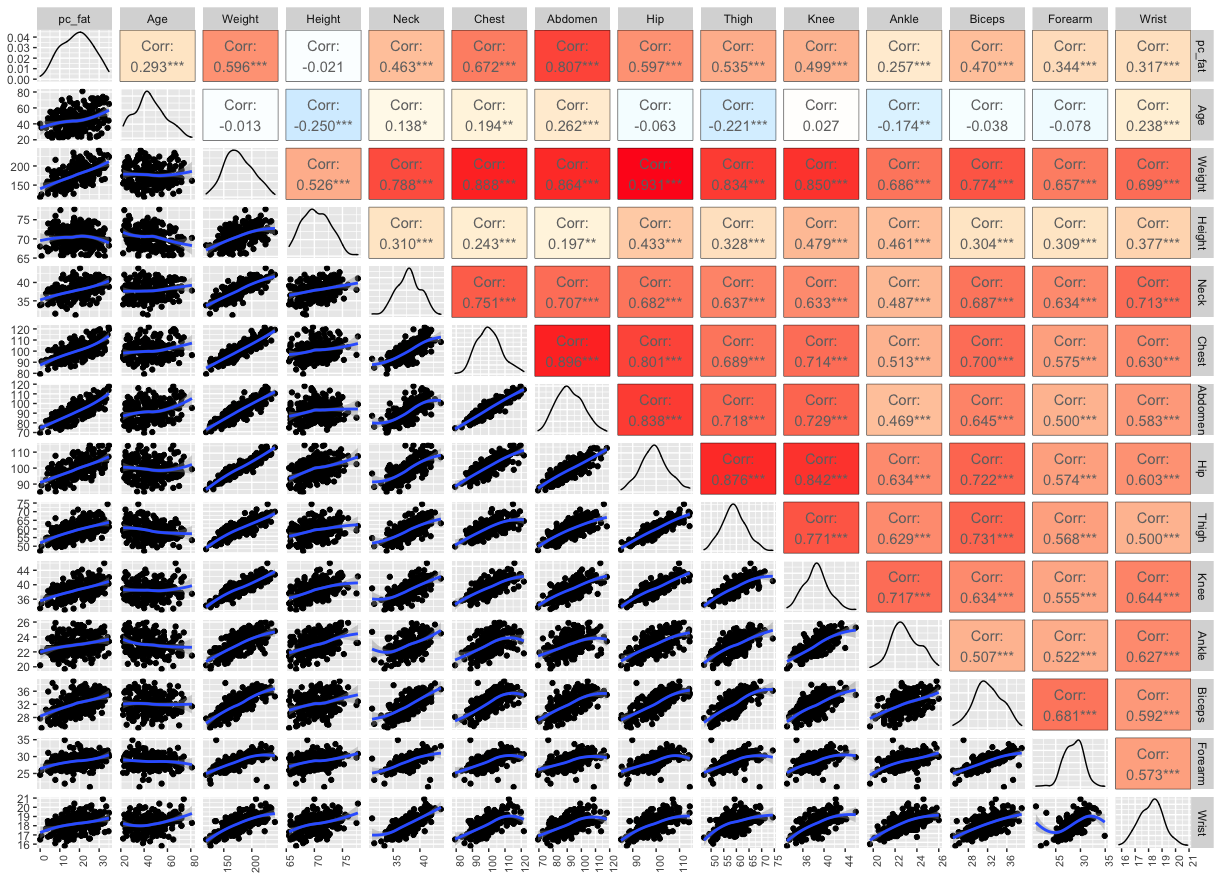
\includegraphics[scale=.40]{pairwise_plot}
	\end{figure}

	\section{Analysis and Results}
	
	The base case linear model is defined as
	\[ Y_{n\times1} =  X_{n\times k}\beta_{k\times1}+\epsilon_{n\times1}\]
	and we present results using variables from the data (the raw data), and from a regression analysis using the estimated principal component's (PCs) \textit{scores} derived from the Principal Components Analysis (PCA).  We first fit a ``Full Model,'' using all $k$ variables from the raw data.  Table~\ref{regression_table1} (1) presents these results, and shows there is an obvious multicollinearity issue present.  This issue is apparent because many of the signs on the estimate coefficients do not match the intuition derived from the pairwise plot analysis.  The multicollinearity concern is further amplified because many variables that are highly correlated with the dependent variable are insignificant.  This problem is not to be ignored, so we employ a Step-Wise Minimal AIC method to reduce the model, discover that the multicollinearity issue persists, then proceed to apply a PCA to reduce the model to PCs, and then use the PC's \textit{scores} in a separate multiple regression to maintain high predictions, enable some level of interpretation, and to finally ward off the multicollinearity issue.
	
	\begin{table}[!htbp] \centering 
		\caption{Initial Multiple Regression Results} 
		\label{regression_table1} 
		\small 
		\begin{tabular}{@{\extracolsep{5pt}}lD{.}{.}{-3} D{.}{.}{-3} } 
			\\[-1.8ex]\hline 
			\hline \\[-1.8ex] 
			& \multicolumn{2}{c}{\textit{Dependent variable:}} \\ 
			\cline{2-3} 
			\\[-1.8ex] & \multicolumn{2}{c}{pc\_fat} \\ 
			\\[-1.8ex] & \multicolumn{1}{c}{(1) Full Model} & \multicolumn{1}{c}{(2) Optimal Step-Wise Model}\\ 
			\hline \\[-1.8ex] 
			Age & 0.063^{*}$ $(0.034) & 0.065^{**}$ $(0.032) \\ 
			Weight & -0.011$ $(0.072) &  \\ 
			Height & -0.241$ $(0.203) & -0.262^{*}$ $(0.139) \\ 
			Neck & -0.385$ $(0.242) & -0.429^{*}$ $(0.220) \\ 
			Chest & -0.112$ $(0.114) &  \\ 
			Abdomen & 0.883^{***}$ $(0.094) & 0.811^{***}$ $(0.071) \\ 
			Hip & -0.202$ $(0.165) & -0.227$ $(0.141) \\ 
			Thigh & 0.219$ $(0.153) & 0.259^{*}$ $(0.138) \\ 
			Knee & -0.030$ $(0.276) &  \\ 
			Ankle & 0.039$ $(0.384) &  \\ 
			Biceps & 0.162$ $(0.176) &  \\ 
			Forearm & 0.291$ $(0.211) & 0.311$ $(0.194) \\ 
			Wrist & -1.593^{***}$ $(0.576) & -1.615^{***}$ $(0.509) \\ 
			Constant & 2.253$ $(25.029) & 3.627$ $(8.933) \\ 
			\hline \\[-1.8ex] 
			Observations & \multicolumn{1}{c}{238} & \multicolumn{1}{c}{238} \\ 
			R$^{2}$ & \multicolumn{1}{c}{0.721} & \multicolumn{1}{c}{0.718} \\ 
			Adjusted R$^{2}$ & \multicolumn{1}{c}{0.705} & \multicolumn{1}{c}{0.708} \\ 
			F Statistic & \multicolumn{1}{c}{44.552$^{***}$} & \multicolumn{1}{c}{72.973$^{***}$} \\ 
			\hline 
			\hline \\[-1.8ex] 
			\textit{Note:}  & \multicolumn{2}{r}{$^{*}$p$<$0.1; $^{**}$p$<$0.05; $^{***}$p$<$0.01} \\ 
		\end{tabular} 
	\end{table} 
	\noindent
	To address the multicollinearity issue, we first reduce the model based on a Step-Wise Minimal AIC regression technique.  This technique reduces the model with the intent of minimizing AIC.  Using this technique, the model is reduced to the one presented in Table~\ref{regression_table1} (2) and has a minimal AIC of $696.28$.  The multicollinearity issue still persists since coefficient signs still go against intuition.  With this lack of assurance in model fit, we further combat the multicollinearity issue using a PCA. A  PCA reduces the independent variable set's dimensionality, while gaining the useful property of independence between the PCs.  We then interpret the characteristics and loadings for each PC, and perform a new multiple regression to show how the multicollinearity issue can be mitigated using a PCA.\footnote{We understand that a Step-Wise Minimal AIC method and PCA are not the only ways to account for multicollinearity in a multiple regression model, but for this project and analysis, we are using these methods to show how a multivariate technique can help improve multiple regression fit and the ability to take inference.}
	
	We employ a PCA on all the independent variables of interest $X_{n\times k}$ to reduce the dimensionality of the data and to ward off the multicollinearity issue.  PCA's help mitigate multicollinearity issues because they explain the variance-covariance structure of the feature measurements $X_{1}, \dots, X_{p}$ through a few linear combinations that are theoretically independent.  These linear combinations are called \textit{principal components} (PCs) and a PCA finds the PCs that account for the variance in the data.  In a PCA, the first PC is the linear combination that accounts for the most variance in the data, and all other PCs follow a pattern where each PC accounts for more variance in the data than the next PC.  Figure~\ref{fig:pc_plot} shows this trend with the PCs, using all variables of interest $X_{n\times k}$, as the amount of variance explained decreases as we move from PC1 (Comp. 1) to PC9 (Comp. 9).\footnote{Note that we do not plot PC11 through PC13 because the percentage of variance explained for these PCs is very small (0.006,0.005,0.004, respectively).}  This trend is also apparent in Table~\ref{tbl:summary_of_pc} which  presents the Standard Deviation (SD), Proportion of Variance (Variance Prop.), and Cumulative Proportion of Variance (Cumulative Prop.) Explained.  A key metric presented in this table is the Cumulative Proportion of Variance Explained (Cumulative Prop.). This metric gives the proportion of variance explained by the first $k$ PCs, and it is useful because if we as researchers are trying to preserve the variance-covariance structure of the feature set $X_{n\times k}$, then we would like to use enough of the PCs in the next multiple regression analysis that explains this  variance-covariance structure.  Figure~\ref{fig:pc_plot} and Table~\ref{tbl:summary_of_pc} indicates that using 5 PCs in the multiple regression analysis may be sufficient as they explain approximately $90 \%$ (exactly $89.7 \%$) of the variance in the data.\footnote{When doing a PCA it is important to use the correlation matrix, instead of the variance-covariance matrix, because some features with large variances could dominate in the PCA.  This could lead to unequal explanation of the variance structure, and therefore, we use the correlation matrix.}
		
	\begin{figure}[!htbp]\centering
		\caption{Principal Component Variance Explanation Plot}
		\label{fig:pc_plot}
		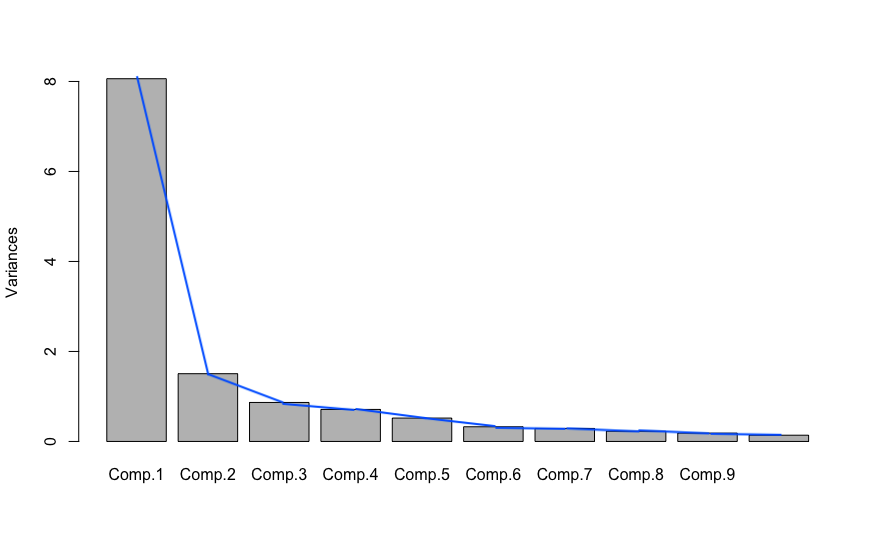
\includegraphics[scale=.40]{pc_out}
	\end{figure}
	

	\begin{table}[!htbp]
		\caption{Summary of PC Variance Explanation} 
		\label{tbl:summary_of_pc} 
		\resizebox{\textwidth}{!}{%
			\begin{tabular}{@{}cccccccccccccc@{}}
				\toprule
				& PC1 & PC2 & PC3 & PC4 & PC5 & PC6 & PC7 & PC8 & PC9 & PC10 & PC11 & PC12 & PC13 \\ \midrule
				SD & 2.839 & 1.227 & 0.931 & 0.844 & 0.721 & 0.571 & 0.538 & 0.476 & 0.431 & 0.373 & 0.290 & 0.257 & 0.137 \\
				\begin{tabular}[c]{@{}c@{}}Variance \\ Prop.\end{tabular} & 0.620 & 0.116 & 0.067 & 0.055 & 0.040 & 0.025 & 0.022 & 0.017 & 0.014 & 0.011 & 0.006 & 0.005 & 0.001 \\
				\begin{tabular}[c]{@{}c@{}}Cumulative \\ Prop.\end{tabular} & 0.620 & 0.736 & 0.803 & 0.857 & 0.897 & 0.922 & 0.945 & 0.962 & 0.976 & 0.987 & 0.993 & 0.999 & 1.000 \\ \bottomrule
			\end{tabular}%
		}
	\end{table}
	\noindent
	Taking a deeper dive into the interpretation of these two PCs, we investigate the loadings $\boldsymbol{\beta}_{i}$ that govern the linear combination for each PC $y_{i}$.  Each PC $y_{i}$ takes on the form of
	\[ y_{i} = \beta_{i1}X_{1} + \dots + \beta_{ik}X_{k} + \dots + \beta_{im}X_{m} \]
	where $\beta_{ik}$ is the loading for feature $X_{k}$, and $i$ is the PC derived from the PCA.  Loadings are important in interpreting PCs because each vector of loadings $\boldsymbol{\beta}_{i}$ contains the coefficients for each variable $X_{k}$ in that linear combination.  Each loading $\beta_{ik}$ represents a relative level of correlation between the PC $y_{i}$ and $X_{ik}$ in that linear combination.  The greater the magnitude of the loading, the higher the correlation between PC $y_{i}$ and feature $X_{k}$.  Table~\ref{tbl:pc_loadings} presents these loadings for all 13 features used in the initial multiple regression, and we find that the first five principal components (PC1-PC5) can be interpreted very differently.  PC1 seems to represent how all the features are positively correlated with each other since all loading signs are positive.  Further note that the smallest loading is \textit{Age}, implying that PC1 is highly correlated with all of the other variables that relate to physical body part measurements.  On the contrary, PC2's highest loading is \textit{Age} implying that PC2 is highly correlated with \textit{Age}, and that the variance in \textit{Age} is most likely being explained by this PC.  The third PC (PC3) seems to account for the variance that is mostly explained by the contrast between \textit{Height \& Wrist} and \textit{Thigh \& Abdomen}.  The forth PC (PC4) seems to account for the variance that is explained by the negative relationship of the arms \textit{Biceps, Forearm \& Wrist} with the rest of the body, and the fifth PC (PC5) seems to account for the variance that is explained by the contrast of the legs \textit{Thigh, Knee \& Ankle} with the rest of the body.  Practitioners should use these loadings interpretations when constructing their own PCA and multiple regression.

	\begin{table}[!htbp] \centering 
		\caption{Principal Component Loadings}
		\label{tbl:pc_loadings} 
		\small
		\resizebox{\textwidth}{!}{%
		\begin{tabular}{@{\extracolsep{-16pt}} D{.}{.}{-3} D{.}{.}{-3} D{.}{.}{-3} D{.}{.}{-3} D{.}{.}{-3} D{.}{.}{-3} D{.}{.}{-3} D{.}{.}{-3} D{.}{.}{-3} D{.}{.}{-3} D{.}{.}{-3} D{.}{.}{-3} D{.}{.}{-3} D{.}{.}{-3} } 
			\\[-1.8ex]\hline 
			\hline \\[-1.8ex] 
			\multicolumn{1}{c}{} & \multicolumn{1}{c}{PC1} & \multicolumn{1}{c}{PC2} & \multicolumn{1}{c}{PC3} & \multicolumn{1}{c}{PC4} & \multicolumn{1}{c}{PC5} & \multicolumn{1}{c}{PC6} & \multicolumn{1}{c}{PC7} & \multicolumn{1}{c}{PC8} & \multicolumn{1}{c}{PC9} & \multicolumn{1}{c}{PC10} & \multicolumn{1}{c}{PC11} & \multicolumn{1}{c}{PC12} & \multicolumn{1}{c}{PC13} \\ 
			\hline \\[-1.8ex] 
			\multicolumn{1}{c}{Age} & 0.006 & 0.730 & 0.364 & 0.124 & 0.007 & 0.324 & 0.206 & 0.131 & 0.217 & 0.276 & 0.116 & 0.131 & 0.037 \\ 
			\multicolumn{1}{c}{Weight} & 0.344 & -0.022 & -0.020 & 0.130 & -0.137 & -0.013 & -0.099 & -0.139 & -0.018 & 0.030 & -0.010 & 0.095 & 0.897 \\ 
			\multicolumn{1}{c}{Height} & 0.167 & -0.433 & 0.569 & 0.228 & -0.560 & 0.113 & 0.032 & -0.054 & 0.066 & 0.152 & 0.097 & -0.105 & -0.175 \\ 
			\multicolumn{1}{c}{Neck} & 0.292 & 0.163 & 0.055 & -0.265 & -0.215 & -0.581 & -0.233 & 0.351 & 0.479 & -0.032 & -0.125 & 0.050 & -0.076 \\ 
			\multicolumn{1}{c}{Chest} & 0.309 & 0.232 & -0.144 & 0.100 & -0.114 & -0.023 & -0.295 & -0.495 & -0.006 & -0.280 & 0.520 & 0.234 & -0.267 \\ 
			\multicolumn{1}{c}{Abdomen} & 0.301 & 0.278 & -0.198 & 0.266 & -0.075 & 0.057 & -0.211 & -0.157 & -0.108 & 0.147 & -0.395 & -0.657 & -0.152 \\ 
			\multicolumn{1}{c}{Hip} & 0.326 & -0.051 & -0.173 & 0.256 & -0.035 & 0.049 & 0.037 & 0.131 & -0.257 & 0.204 & -0.434 & 0.651 & -0.233 \\ 
			\multicolumn{1}{c}{Thigh} & 0.302 & -0.155 & -0.355 & 0.116 & 0.116 & -0.068 & 0.212 & 0.371 & -0.039 & 0.443 & 0.562 & -0.173 & -0.038 \\ 
			\multicolumn{1}{c}{Knee} & 0.310 & -0.057 & 0.090 & 0.275 & 0.198 & 0.266 & 0.090 & 0.443 & 0.067 & -0.699 & 0.006 & -0.101 & -0.010 \\ 
			\multicolumn{1}{c}{Ankle} & 0.258 & -0.259 & 0.253 & 0.035 & 0.683 & 0.019 & -0.087 & -0.311 & 0.415 & 0.211 & -0.092 & 0.022 & -0.060 \\ 
			\multicolumn{1}{c}{Biceps} & 0.290 & -0.003 & -0.195 & -0.336 & -0.174 & 0.060 & 0.742 & -0.314 & 0.200 & -0.131 & -0.142 & -0.050 & -0.047 \\ 
			\multicolumn{1}{c}{Forearm} & 0.256 & -0.067 & -0.002 & -0.667 & -0.044 & 0.563 & -0.350 & 0.147 & -0.112 & 0.097 & 0.004 & -0.007 & -0.022 \\ 
			\multicolumn{1}{c}{Wrist} & 0.270 & 0.143 & 0.462 & -0.228 & 0.225 & -0.377 & 0.158 & -0.018 & -0.641 & -0.041 & 0.054 & -0.085 & -0.015 \\ 
			\hline \\[-1.8ex] 
		\end{tabular}
	}
	\end{table} 
	\noindent
	It is clear that we have an interpretation for these PCs and that we can use them to explain approximately $90 \%$ of the variance for the features we are using to explain a person's \% \textit{percent body fat}.  With that said, we then use the \textit{scores} from each PC in a multiple regression to help explain a person's body fat percentage, and the results are reported in Table~\ref{regression_table2}.  Each \textit{score} for each PC is derived by plugging in the observational data values $\textbf{x}_{1},\dots,\textbf{x}_{N}$ into each one of estimated linear functions that make up each $y_{i}$.  We report 3 linear regression models in Table~\ref{regression_table2}, and show how we have warded off the multicollinearity issue in Figure~\ref{fig:scores_plot}.  In all three models, all coefficients are significant in explaining \textit{percent body fat} with the exception of Comp.5 in model (3), and it is now valid to take inference from these coefficients since all models satisfy the equal variance and normality assumptions (p-values = $\left[(0.2285,0.4446,0.6142),(0.1918,0.3632,0.1106)\right]$ ), and it is clear through Figure~\ref{fig:scores_plot} that all PCs exhibit independence since correlations are close to zero and the plots seem to not have a clear positive or negative trend. \footnote{The Durbin-Watson AR1 auto-correlation test is rejected ( p-value = $(0.0004157,0.003026,0.002731)$), but not by that much in the second regression, and we do not think that not fully satisfying this assumption invalidates results.}  We propose using the Model (3) PC1-PC5 because it has a reasonably high $R^{2} = 0.630$, it incorporates all measurements taken on a person's body, it explains approximately $90 \%$ of the variance in the explanatory variables, and more importantly, it wards off the initial multicollinearity issue we encountered in the first multiple regression analyses.  Each coefficient effect can be interpreted using the intuition derived from the paragraph above which shows that the first coefficient accounts for all body measurements, the second seems to account for age, the third represents how the contrast between \textit{Height \& Wrist} and \textit{Thigh \& Abdomen} have a negative effect on an individuals body fat percentage, and similar interpretation can be used for the estimated coefficients on PC4 and PC5.
	\begin{table}[!htbp] \centering 
		\caption{Principal Component Regression Results} 
		\label{regression_table2} 
		\small 
		\begin{tabular}{@{\extracolsep{-25pt}}lD{.}{.}{-3} D{.}{.}{-3} D{.}{.}{-3} } 
			\\[-1.8ex]\hline 
			\hline \\[-1.8ex] 
			& \multicolumn{3}{c}{\textit{Dependent variable:}} \\ 
			\cline{2-4} 
			\\[-1.8ex] & \multicolumn{3}{c}{pc\_fat} \\ 
			\\[-1.8ex] & \multicolumn{1}{c}{(1) PC1} & \multicolumn{1}{c}{(2) PC1-PC3} & \multicolumn{1}{c}{(3) PC1-PC5}\\ 
			\hline \\[-1.8ex] 
			Comp.1 & 1.629^{***}$ $(0.145) & 1.629^{***}$ $(0.116) & 1.629^{***}$ $(0.110) \\ 
			Comp.2 &  & 2.490^{***}$ $(0.267) & 2.490^{***}$ $(0.255) \\ 
			Comp.3 &  & -2.510^{***}$ $(0.352) & -2.510^{***}$ $(0.336) \\ 
			Comp.4 &  &  & 1.867^{***}$ $(0.371) \\ 
			Comp.5 &  &  & -0.204$ $(0.434) \\ 
			Constant & 18.705^{***}$ $(0.412) & 18.705^{***}$ $(0.328) & 18.705^{***}$ $(0.313) \\ 
			\hline \\[-1.8ex] 
			Observations & \multicolumn{1}{c}{238} & \multicolumn{1}{c}{238} & \multicolumn{1}{c}{238} \\ 
			R$^{2}$ & \multicolumn{1}{c}{0.348} & \multicolumn{1}{c}{0.590} & \multicolumn{1}{c}{0.630} \\ 
			Adjusted R$^{2}$ & \multicolumn{1}{c}{0.346} & \multicolumn{1}{c}{0.584} & \multicolumn{1}{c}{0.622} \\ 
			Residual Std. Error & \multicolumn{1}{c}{6.349} & \multicolumn{1}{c}{5.061} & \multicolumn{1}{c}{4.823} \\ 
			F Statistic & \multicolumn{1}{c}{126.206$^{***}$ } & \multicolumn{1}{c}{112.036$^{***}$} & \multicolumn{1}{c}{79.128$^{***}$} \\ 
			\hline 
			\hline \\[-1.8ex] 
			\textit{Note:}  & \multicolumn{3}{r}{$^{*}$p$<$0.1; $^{**}$p$<$0.05; $^{***}$p$<$0.01} \\ 
		\end{tabular} 
	\end{table} 	
	\begin{figure}[!htbp]\centering
		\caption{Pairwise Plot of PC Scores}
		\label{fig:scores_plot}
		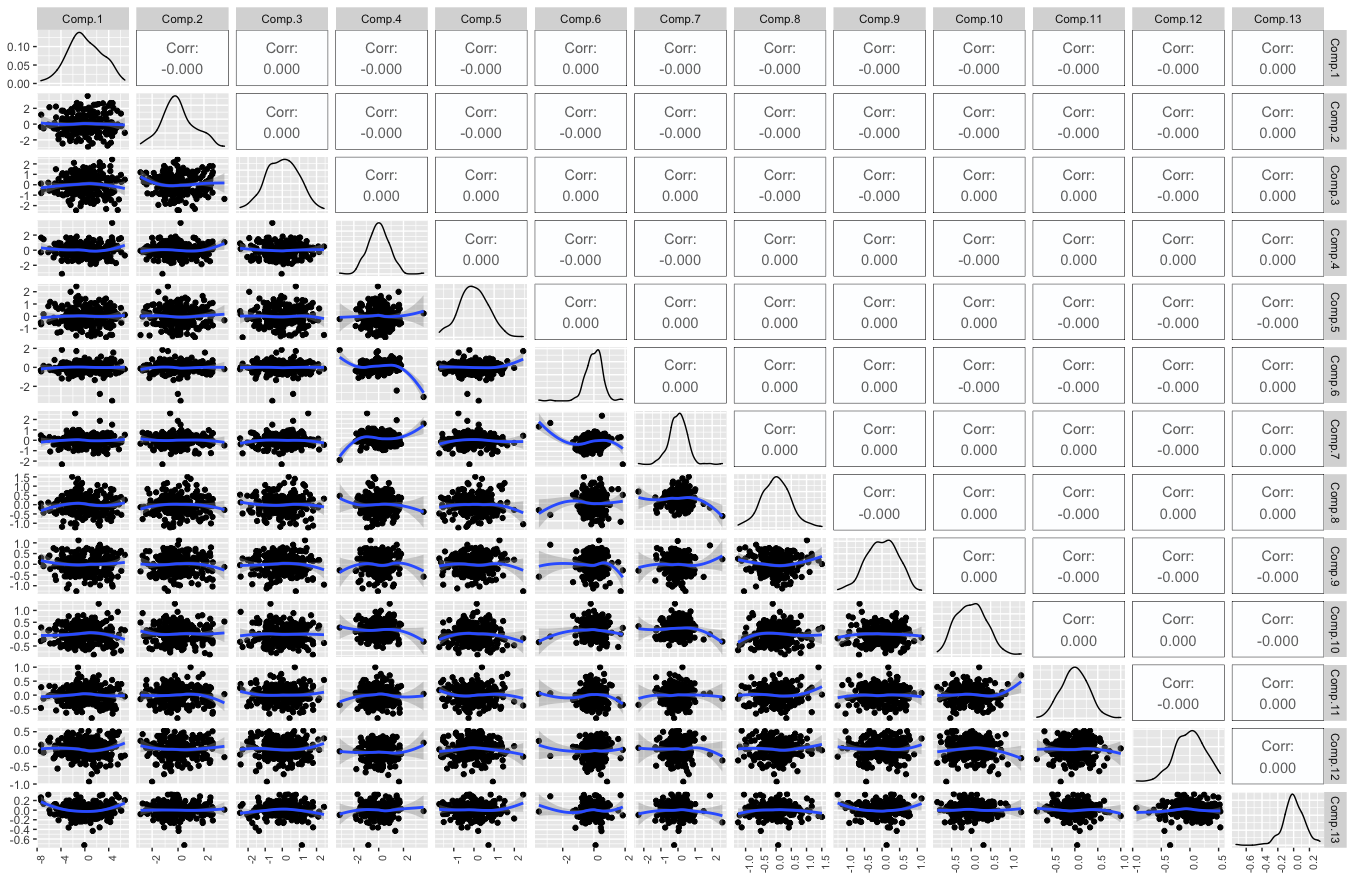
\includegraphics[scale=.37]{PCPlot.png}
	\end{figure}
	\section{Conclusion}
	We show a method to predict the body fat percentage of an individual in the presences of multicollinearity using a model with a large set of features.  To do this, we reduce the diminsionaltiy dataset using PCA, and use the first five PCs to predict body fat percentage with the support of inference and interpretation.  This research is important because practitioners can use this methodology to first derive their own models for prediction, and then use the loadings and multiple regression coefficients to quickly predict a person's body fat percentage.  We also show that PCA can be useful in curtain circumstances where other methods are not great at dealing with multicollinearity, such as the Step-Wise Minimal AIC method.  We hope our insights will reduce costs in estimating a person's body fat percentage.

	\pagebreak
	
	\section{References}
	
	\begin{itemize}
		\item Bailey, Covert (1994). Smart Exercise: Burning Fat, Getting Fit,
		Houghton-Mifflin Co., Boston, pp. 179-186.
		
		\item Behnke, A.R. and Wilmore, J.H. (1974). Evaluation and Regulation of Body
		Build and Composition, Prentice-Hall, Englewood Cliffs, N.J.
		
		\item Siri, W.E. (1956), "Gross composition of the body", Advances in 
		Biological and Medical Physics, vol. IV, edited by J.H. Lawrence and C.A.
		Tobias, Academic Press, Inc., New York.
		
		\item Katch, Frank and McArdle, William (1977). Nutrition, Weight Control, and
		Exercise, Houghton Mifflin Co., Boston.
		
		\item Wilmore, Jack (1976). Athletic Training and Physical Fitness: Physiological
		principals of the Conditioning Process, Allyn and Bacon, Inc., Boston.
	\end{itemize}

\end{document}